\documentclass[varwidth=true, border=0.2in]{standalone}
\usepackage{tikz}
\usepackage[labelfont=normalsize, labelformat=parens, justification=centering]{caption, subfig}

%%%%%%%%%%%%%%%
%%%%%%%%%%%%%%%
\begin{document}

\begin{figure}[htb!]
%%%%%%%%%%%%%%%%
% Experiment 1.1
%%%%%%%%%%%%%%%%
  \subfloat{
    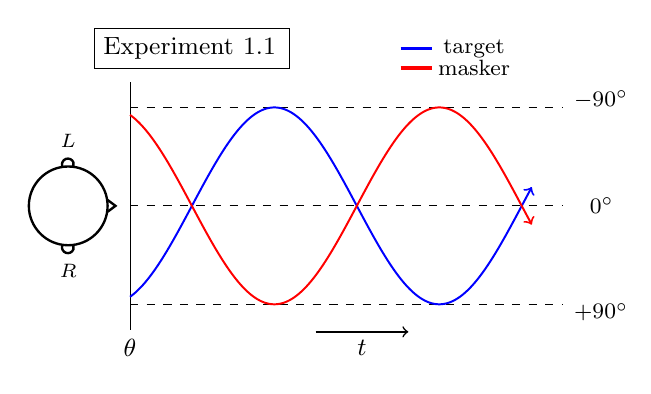
\begin{tikzpicture}
      % Title
      \node[draw, align=left, text width=2.25cm] at (pi/2, 2) {\small Experiment 1.1};
      
      % Legend
      \draw[line width=0.4mm, blue] (43*pi/32, 2.  ) -- (43*pi/32 + pi/8, 2.  );
      \node at (5*pi/4 + 25*pi/64, 2.  ) {\footnotesize target};
      \draw[line width=0.4mm,  red] (43*pi/32, 1.75) -- (43*pi/32 + pi/8, 1.75);
      \node at (5*pi/4 + 25*pi/64, 1.75) {\footnotesize masker};
      
      % y axis
      \draw[line width=0.125mm, black] (pi/4, -1.575) -- (pi/4, 1.575);
      \node at (pi/4, -1.8) {\small $\theta$};
      
      % Dashed degree guide lines
      \draw[line width=0.125mm, black, dashed] (pi/4,  1.25) -- (2*pi,  1.25);
      \draw[line width=0.125mm, black, dashed] (pi/4,  0.)   -- (2*pi,  0.  );
      \draw[line width=0.125mm, black, dashed] (pi/4, -1.25) -- (2*pi, -1.25);
      
      % Degree guides
      \node[align=right, text width=0.5cm] at (2*pi + pi/8,  1.35)
        {\footnotesize $-90^{\circ}$};
      \node[align=right, text width=0.5cm] at (2*pi + pi/8,  0.)
        {\footnotesize $0^{\circ}$};
      \node[align=right, text width=0.5cm] at (2*pi + pi/8, -1.35)
        {\footnotesize $+90^{\circ}$};
      
      % Arrow of time
      \draw[help lines, ->, line width=0.2mm, black] (pi, -1.6) -- (11*pi/8, -1.6);
      \node at (19*pi/16, -1.8) {\small $t$};
      
      % Sinusoids
      \draw[help lines, ->, line width=0.25mm, blue, domain=pi/4:2*pi - pi/8, samples=1000]
           plot(\x, {-1.25*sin((1.5*\x + pi/4) r)});
      \draw[help lines, ->, line width=0.25mm,  red, domain=pi/4:2*pi - pi/8, samples=1000]
           plot(\x, { 1.25*sin((1.5*\x + pi/4) r)});
      
      % Head
      \node at (0, 0.825) {\scriptsize $L$};
      \draw[line width=0.3mm] (0, 0) circle (0.5cm); % head
      \draw[line width=0.3mm] (0 - 0.075,  0.5) arc ( 200:-20:0.075); % R ear
      \draw[line width=0.3mm]
             (0 + 0.5,  0.075) --
             (0 + 0.6,  0.   ) --
             (0 + 0.5, -0.075); % nose
      \draw[line width=0.3mm] (0 - 0.075, -0.5) arc (-200: 20:0.075); % L ear
      \node at (0, -0.825) {\scriptsize $R$};
    \end{tikzpicture}
  }
%%%%%%%%%%%%%%%


%%%%%%%%%%%%%%%
% Experiment 2
%%%%%%%%%%%%%%%
  \subfloat{
    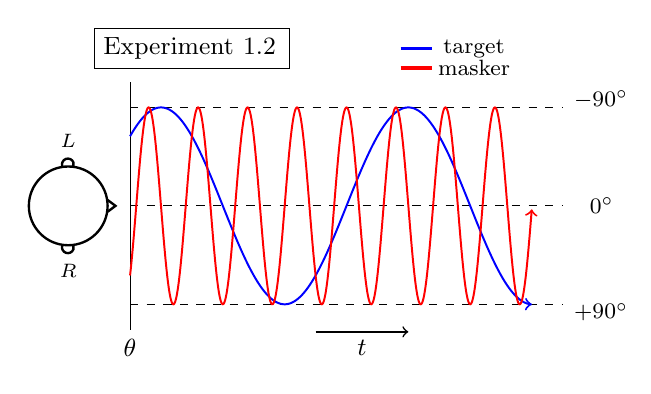
\begin{tikzpicture}
      % Title
      \node[draw, align=left, text width=2.25cm] at (pi/2, 2) {\small Experiment 1.2};
      
      % Legend
      \draw[line width=0.4mm, blue] (43*pi/32, 2.  ) -- (43*pi/32 + pi/8, 2.  );
      \node at (5*pi/4 + 25*pi/64, 2.  ) {\footnotesize target};
      \draw[line width=0.4mm,  red] (43*pi/32, 1.75) -- (43*pi/32 + pi/8, 1.75);
      \node at (5*pi/4 + 25*pi/64, 1.75) {\footnotesize masker};
      
      % y axis
      \draw[line width=0.125mm, black] (pi/4, -1.575) -- (pi/4, 1.575);
      \node at (pi/4, -1.8) {\small $\theta$};
      
      % Dashed degree guide lines
      \draw[line width=0.125mm, black, dashed] (pi/4,  1.25) -- (2*pi,  1.25);
      \draw[line width=0.125mm, black, dashed] (pi/4,  0.)   -- (2*pi,  0.  );
      \draw[line width=0.125mm, black, dashed] (pi/4, -1.25) -- (2*pi, -1.25);
      
      % Degree guides
      \node[align=right, text width=0.5cm] at (2*pi + pi/8,  1.35)
        {\footnotesize $-90^{\circ}$};
      \node[align=right, text width=0.5cm] at (2*pi + pi/8,  0.)
        {\footnotesize $0^{\circ}$};
      \node[align=right, text width=0.5cm] at (2*pi + pi/8, -1.35)
        {\footnotesize $+90^{\circ}$};
      
      % Arrow of time
      \draw[help lines, ->, line width=0.2mm, black] (pi, -1.6) -- (11*pi/8, -1.6);
      \node at (19*pi/16, -1.8) {\small $t$};
      
      % Sinusoids
      \draw[help lines, ->, line width=0.25mm, blue, domain=pi/4:2*pi - pi/8, samples=1000]
           plot(\x, {1.25*sin(( 2*\x - pi/4) r)});
      \draw[help lines, ->, line width=0.25mm,  red, domain=pi/4:2*pi - pi/8, samples=1000]
           plot(\x, {1.25*sin((10*\x - 3*pi/4) r)});
      
      % Head
      \node at (0, 0.825) {\scriptsize $L$};
      \draw[line width=0.3mm] (0, 0) circle (0.5cm); % head
      \draw[line width=0.3mm] (0 - 0.075,  0.5) arc ( 200:-20:0.075); % R ear
      \draw[line width=0.3mm]
             (0 + 0.5,  0.075) --
             (0 + 0.6,  0.   ) --
             (0 + 0.5, -0.075); % nose
      \draw[line width=0.3mm] (0 - 0.075, -0.5) arc (-200: 20:0.075); % L ear
      \node at (0, -0.825) {\scriptsize $R$};
    \end{tikzpicture}
  }
%%%%%%%%%%%%%%%
\caption*{hello!}
\end{figure}

%%%%%%%%%%%%%%%
%%%%%%%%%%%%%%%
\end{document}
